\uuid{LcjB}
\exo7id{5050}
\titre{exo7 5050}
\auteur{quercia}
\organisation{exo7}
\datecreate{2010-03-17}
\isIndication{false}
\isCorrection{true}
\chapitre{Surfaces}
\sousChapitre{Surfaces paramétrées}
\module{Géométrie}
\niveau{L2}
\difficulte{}

\contenu{
\texte{
Dessiner la surface ${\cal S}$ d'équations paramétriques :
$\begin{cases} x = a\cos u/\ch v\cr
         y = a\sin u/\ch v\cr
         z = a(v-\tanh v)\cr \end{cases}$
où $a$ est un réel strictement positif (pseudo-sphère).
}
\reponse{
$$
\centerline{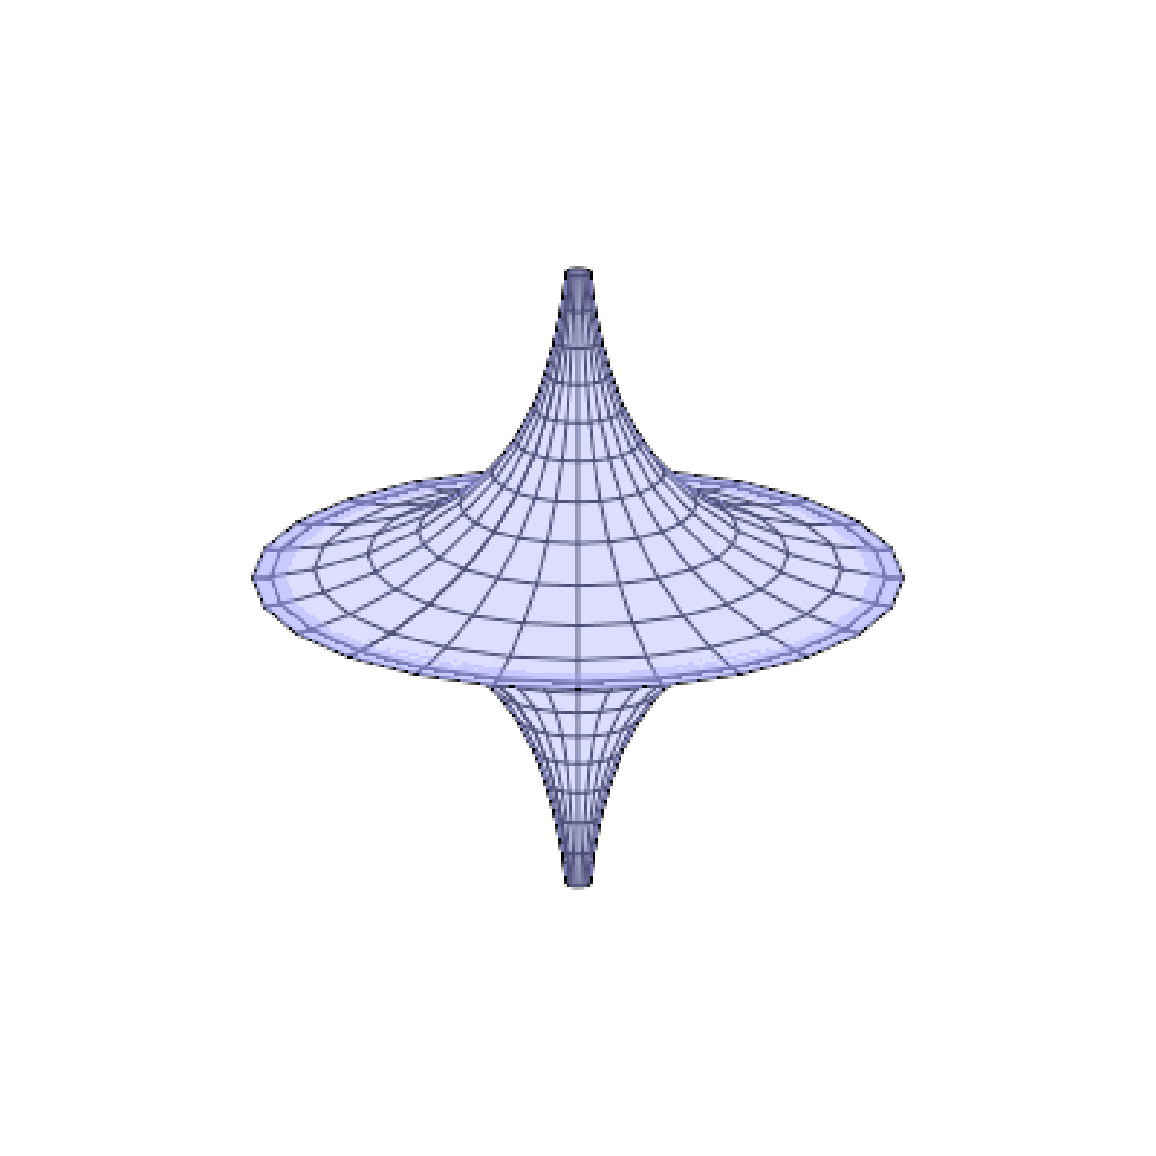
\includegraphics[height=6cm]{../images/pdf/LcjB-1.pdf}}
$$
% \mapleplot{%
% x := cos(u)/cosh(v); y := sin(u)/cosh(v); z := v-tanh(v);
% plot3d([x,y,z],u=0..2*Pi,v=-4..4,style=hidden,color=black,orientation=[45,70]);}
}
}
